\newcommand{\parallelsum}{\mathbin{\!/\mkern-5mu/\!}}

\section{Circuit}

Figure \ref{fig:circuit} shows the circuit chosen.
This circuit was chosen due to it having two stages, helping increase the gain.

\begin{figure}[h]
	\centering
	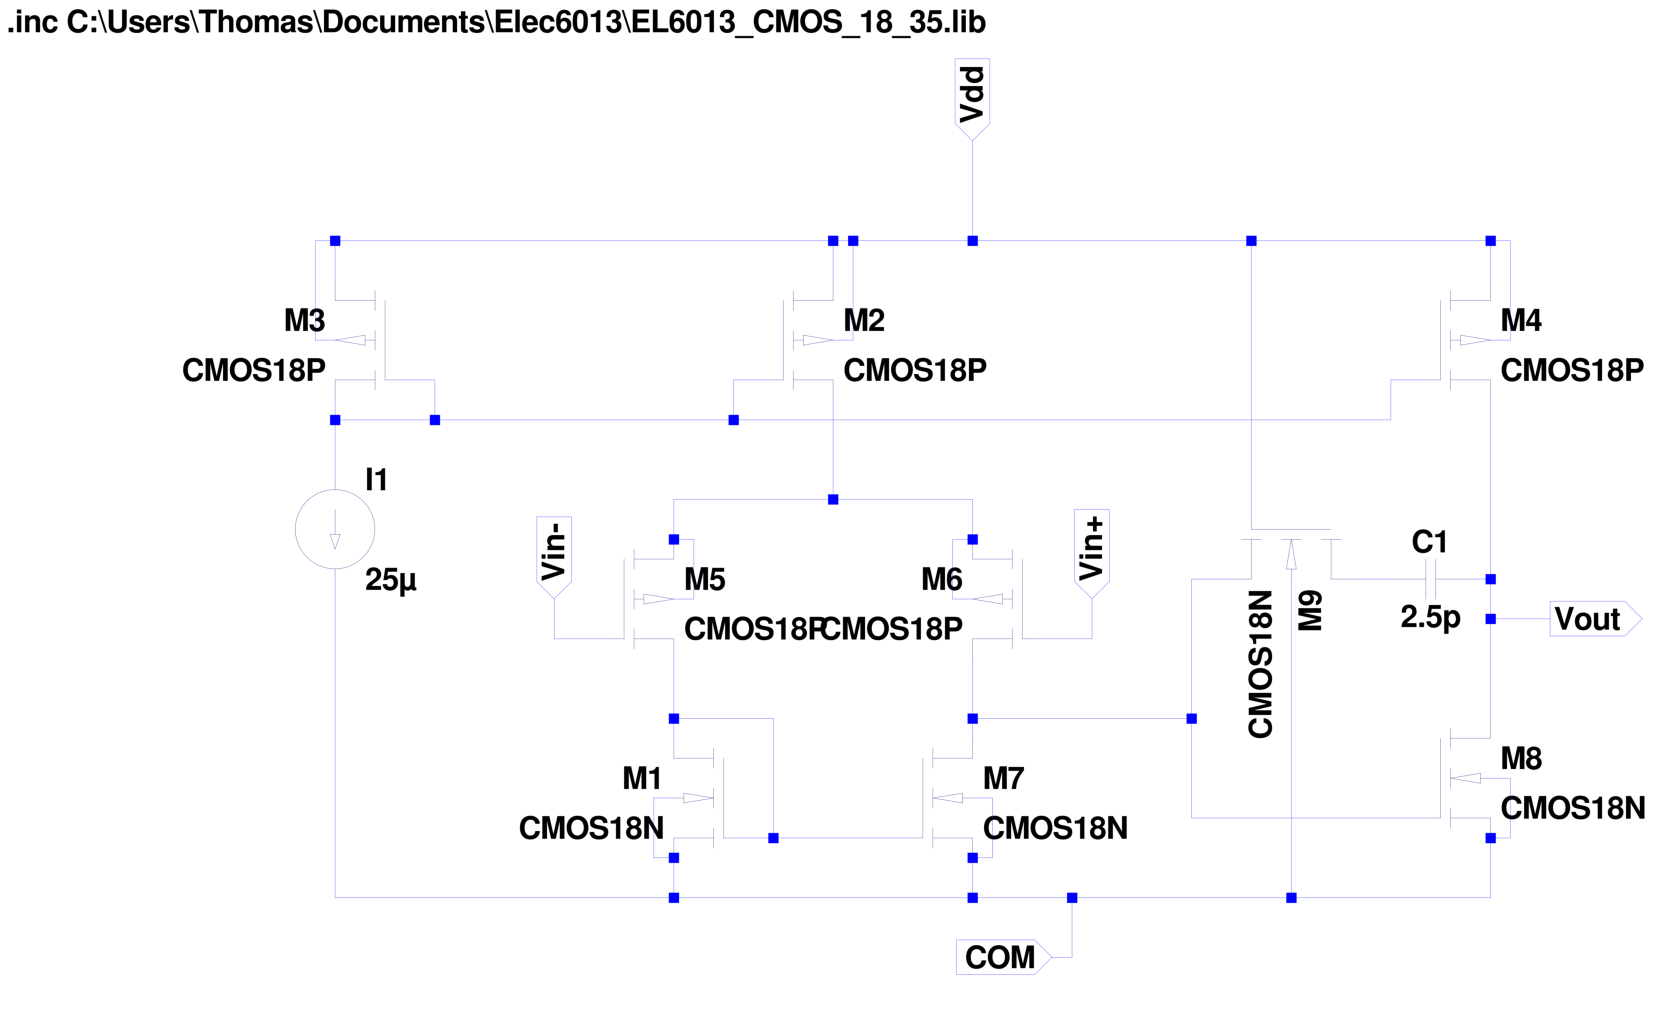
\includegraphics[width=0.75\textwidth]{./images/coursework.pdf}
	\caption{The chosen circuit}
	\label{fig:circuit}
\end{figure}

\section{Design calculations}

The first calculation done was to determine the required minimum unity gain frequency ($\omega_{0dB}$), as this would help define pole frequencies.
This was done using the knowledge of the minimum required gain at the full power frequency, this gave a corner frequency beyond which the gain would be dropping off at a rate of $20dB$ per decade.

Using standard straight line equation: \\
$y = mx+c$ \\
$m = \frac{\Delta y}{\Delta x}$ \\
$m = \frac{26 - 6}{\num{100e3} - \num{1e6}}$ \\
$m = \num{-22.22e-6}$\\

$\omega_{0dB} = \frac{A_{0} - A_{c}}{m} + \omega_{c}$ \\
$\omega_{0dB} = \frac{0 - 26}{\num{-22.22e-6}} + \num{2\pi e5}$ \\
$\omega_{0dB} = 1798318.531 rad/s$ \\

Secondly we determine the value for the gain.

$A_{dB} = 20 log(A_{v})$ \\
$A_{v} = 10^{\frac{A_{dB}}{20}}$ \\
$A_{v} = 10^{\frac{60}{20}}$ \\
$A_{v} = 1000$ \\

\subsection{Stage 2}

Both poles in the amplifier need to be above $100KHz$ ($\num{2\pi e5}$).
The pole in the second stage of the op-amp is formed between $M_{8}$ and $C_{L}$.

$P_{2} = \frac{gm_{8}}{C_{L}}$ \\

$P_{2}$ wants to be greater than 2.5 times the unity gain frequency to avoid undesirable phase effects.

$P_{2} = 3 \times \omega_{0dB}$ \\
$P_{2} = 3 \times 1798318.531$ \\
$P_{2} = 5394955.592 rad/s$ \\

$gm_{8} = P_{2}C_{L}$ \\
$gm_{8} = 5394955.592 \times \num{120e-12}$ \\
$gm_{8} = \num{6.474e-4}$ \\

Now $V_{gs} - V_{T}$ needs to be defined.
For the transistors to be in the saturation region it ideally needs to be greater than $0.2V$, however above $0.3V$ will cause the device to not be able to produce the desired output range.

Let $V_{gs} - V_{T} = 0.25V$.

$I_{DS8} = \frac{gm_{8}(V_{gs} - V_{T})}{2}$ \\
$I_{DS8} = \frac{\num{6.474e-4}(0.25)}{2}$ \\
$I_{DS8} = \num{80.925e-6}$ \\

$A_{v} = A_{1}A_{2}$

Let $A_{2} = 10$

$A_{2} = gm_{8}(r_{DS8} \parallelsum r_{DS4})$ \\
$(r_{DS8} \parallelsum r_{DS4}) = \frac{A_{2}}{gm_{8}}$ \\
$(r_{DS8} \parallelsum r_{DS4}) = \frac{1000}{\num{6.474e-4}}$ \\
$(r_{DS8} \parallelsum r_{DS4}) = 15446.40$ \\
$r_{DS8} = r_{DS4}$ \\
$r_{DS8} = 2 \times (r_{DS8} \parallelsum r_{DS4})$ \\
$r_{DS8} = 2 \times 15446.40$ \\
$r_{DS8} = 30892.802$ \\

$r_{DS8} = \frac{L_{8} - 0.03}{0.033I_{DS8}}$ \\
$L_{8} \ge 0.033I_{DS8}r_{DS8} + 0.03$ \\
$L_{8} \ge 0.033 \times \num{80.925e-6} \times 30892.802 + 0.03$ \\
$L_{8} \ge 0.1125$ \\

This is less than $L_{min}$ ($0.18\mu m$).
Let

$L_{8} = 2L_{min}$ 	\\
$L_{8} = 2 \times 0.18$ \\
$L_{8} = 0.36\mu m$ \\

$\frac{W_{8}}{L_{8}} = \frac{{gm_{8}}^{2}n}{2I_{DS8}\mu C_{ox}}$ \\
$\frac{W_{8}}{L_{8}} = \frac{(\num{6.474e-4})^{2} \times 1.3}{2 \times \num{80.925e-6} \times \num{330e-6}}$ \\
$\frac{W_{8}}{L_{8}} = 10.20$ \\

$W_{8} = 10.20L_{8}$ \\
$W_{8} = 10.20 \times 0.36$ \\
$W_{8} = 3.67\mu m$ \\

$r_{DS8} = \frac{L_{8} - 0.03}{0.033I_{DS8}}$ \\
$r_{DS8} = \frac{0.36 - 0.03}{0.033 \times \num{80.925e-6}}$ \\
$r_{DS8} = 123571.21$ \\

$(r_{DS8} \parallelsum r_{DS4}) = \frac{1}{2} \times r_{DS8}$ \\
$(r_{DS8} \parallelsum r_{DS4}) = \frac{1}{2} \times 123571.21$ \\
$(r_{DS8} \parallelsum r_{DS4}) = 61785.6$ \\

$A_{2} = gm_{8}(r_{DS8} \parallelsum r_{DS4})$ \\
$A_{2} = \num{6.474e-4} \times 61785.6$ \\
$A_{2} = 40$ \\

Now the width of $M_{4}$ needs to be determined to ensure the desired current flows through $M_{8}$.
For $r_{DS8}$ to equal $r_{DS4}$ the two transistors must have the same length.

$W_{4} = W_{3}\frac{I_{D4}}{I_{D3}}\frac{L_{4}}{L_{3}}$ \\
$W_{4} = 5\frac{\num{80.925e-6}}{\num{25e-6}}\frac{0.36}{1}$ \\
$W_{4} = 5.8266$ \\

\subsection{Stage 1}
Now we consider the first stage of the amplifier.
So far the following values have been defined for this section:

$V_{gs} - V_{T} = 0.25$ \\

This gives a fair amount of freedom in this design stage.
Firstly the tail current is defined:

$I_{T} = \num{200e-6}A$ \\

Let $L_{2} = 1\mu m$ \\

$W_{2} = W_{3}\frac{I_{D2}}{I_{D3}}\frac{L_{2}}{L_{3}}$ \\
$W_{2} = 5\frac{\num{100e-6}}{\num{25e-6}}\frac{1}{1}$ \\
$W_{2} = 40$ \\

$gm_{6} = \frac{2I_{DS6}}{V_{gs} - V_{T}}$ \\
$gm_{6} = \frac{2 \times \frac{1}{2}I_{T}}{V_{gs} - V_{T}}$ \\
$gm_{6} = \frac{2 \times \frac{1}{2} \times \num{200e-6}}{0.25}$ \\
$gm_{6} = \num{8e-4}$ \\

$A_{1} = \frac{A_{v}}{A_{2}}$ \\
$A_{1} = \frac{1000}{10}$ \\
$A_{1} = 100$ \\

$A_{1} = gm_{6}(r_{DS6} \parallelsum r_{DS7})$ \\
$(r_{DS6} \parallelsum r_{DS7}) = \frac{A_{1}}{gm_{6}}$ \\
$(r_{DS6} \parallelsum r_{DS7}) = \frac{100}{\num{8e-4}}$ \\
$(r_{DS6} \parallelsum r_{DS7}) = 125000$ \\

$r_{DS6} = r_{DS7}$ \\
$r_{DS6} = 2(r_{DS6} \parallelsum r_{DS7})$ \\
$r_{DS6} = 2 \times 125000$ \\
$r_{DS6} = 250000$ \\

$L_{6} \ge 0.033I_{DS6}r_{DS6} + 0.03$ \\
$L_{6} \ge 0.033 \times \num{100e-6} \times 250000 + 0.03$ \\
$L_{6} \ge 0.855\mu m$ \\

Let $L_{6} = 1\mu m$

$r_{DS6} = \frac{L_{6} - 0.03}{0.033I_{DS6}}$ \\
$r_{DS6} = \frac{1 - 0.03}{0.033 \times \num{100e-6}}$ \\
$r_{DS6} = 293939.39$ \\

$(r_{DS6} \parallelsum r_{DS7}) = \frac{1}{2}r_{DS6}$ \\
$(r_{DS6} \parallelsum r_{DS7}) = \frac{1}{2} \times 293939.39$ \\
$(r_{DS6} \parallelsum r_{DS7}) = 146969.697$ \\

$A_{1} = gm_{6}(r_{DS6} \parallelsum r_{DS7})$ \\
$A_{1} = \num{8e-4} \times 146969.697$ \\
$A_{1} = 117.57$ \\

This gives a potential value to $A_{v}$ of:

$A_{v} = A_{1}A_{2}$ \\
$A_{v} = 117.57 \times 40$ \\
$A_{v} = 4702.8$ \\

$A_{dB} = 20log(A_{v})$ \\
$A_{dB} = 20log(4702.8)$ \\
$A_{dB} = 73.44dB$ \\

$gm_{6} = \sqrt{\frac{2I_{DS6}\mu C_{ox}W_{6}}{nL_{6}}}$ \\
$\frac{W_{6}}{L_{6}} = \frac{gm_{6}^{2}n}{2I_{DS6}\mu C_{ox}}$ \\
$\frac{W_{6}}{L_{6}} = \frac{(\num{8e-4})^{2} \times 1.3}{2 \times \num{100e-6} \times \num{100e-6}}$ \\
$\frac{W_{6}}{L_{6}} = 41.6$ \\

$W_{6} = 41.6L_{6}$ \\
$W_{6} = 41.6 \times 1$ \\
$W_{6} = 41.6\mu m$ \\

We now consider the current mirror.

$L_{1} = L_{7}$ \\
$W_{1} = L_{7}$ \\

For $V_{gs} - V_{T} = 0.25$ we get $gm = \num{8e-4}$.

$\frac{W_{1}}{L_{1}} = \frac{gm_{6}^{2}n}{2I_{DS1}\mu C_{ox}}$ \\
$\frac{W_{1}}{L_{1}} = \frac{(\num{8e-4})^{2} \times 1.3}{2 \times \num{100e-6} \times \num{330e-6}}$ \\
$\frac{W_{1}}{L_{1}} = 12.61$ \\

Let $L_{1} = L_{6}$ so that $r_{DS1} = r_{DS6}$ 

$L_{1} = 1\mu m$ \\
$W_{1} = 12.61 \times L_{1}$ \\
$L_{1} = 12.61 \times 1$ \\
$L_{1} = 12.61\mu m$ \\

\subsection{Compensation}

Now that the two gain stages of the op-amp have been considered the feedback loop needs consideration.
This capacitor creates a pole with $gm_{6}$, which needs to be above the unity gain frequency $\omega_{0dB}$.

$\omega_{dB} = \frac{gm_{6}}{C_{Cmax}}$ \\
$C_{Cmax} = \frac{gm_{6}}{\omega_{0dB}}$ \\
$C_{Cmax} = \frac{\num{8e-4}}{1798313.531}$ \\
$C_{Cmax} = \num{444.86e-12}$ \\
$C_{Cmax} = \num{444.86e-12}pF$ \\

This is a rather large value for an on-chip capacitance, and a reduction in it will distance it from the minimum unity gain frequency.

Let $C_{C} = 2.5pF$, as this is much more realisable and dractically raises the frequency of the pole.

Now $r_{DS9}$ needs to be set to cancel the zero.

$r_{DS9} = \frac{1}{gm_{6}}$ \\
$r_{DS9} = \frac{1}{\num{8e-4}}$ \\
$r_{DS9} = 1250$ \\

$r_{DS9} = \frac{L_{9}}{\mu_{Eff}C_{ox}W_{9}(V_{gs} - V_{T})}$ \\

Using

$\mu = \frac{\mu C_{ox}}{C_{ox}}$

and

$\mu_{Eff} = \frac{\mu}{1 + \theta (V_{gs} - V_{T})}$ \\

$r_{DS9} = \frac{L_{9}(1 + \theta (V_{gs} - V_{T}))}{\mu C_{ox}W_{9}(V_{gs} - V_{T})}$ \\
$\frac{W_{9}}{L_{9}} = \frac{1 + \theta (V_{gs} - V_{T})}{\mu C_{ox}r_{DS9}(V_{gs} - V_{T})}$ \\
$\frac{W_{9}}{L_{9}} = \frac{1 + 0.6(0.25)}{\num{330e-6} \times 1250 \times 0.25}$ \\
$\frac{W_{9}}{L_{9}} = 11.15$ \\

$L_{9} = 1\mu m$ \\
$W_{9} = 11.15\mu m$ \\

We have now determined values for all the components in the design.
The following table shows all the component values.

\begin{table}[h]
	\begin{tabular}{| l | l | l |}
		\hline
		Device			& Variable	& Value		\\
		\hline
		\multirow{2}{*}{M1}	& L		& $12.61\mu m$	\\
					& W		& $1\mu m$	\\
		\hline
		\multirow{2}{*}{M2}	& L		& $40\mu m$	\\
					& W		& $1\mu m$	\\
		\hline
		\multirow{2}{*}{M3}	& L		& $5\mu m$	\\
					& W		& $1\mu m$	\\
		\hline
		\multirow{2}{*}{M4}	& L		& $5.83\mu m$	\\
					& W		& $0.36\mu m$	\\
		\hline
		\multirow{2}{*}{M5}	& L		& $41.6\mu m$	\\
					& W		& $1\mu m$	\\
		\hline
		\multirow{2}{*}{M6}	& L		& $41.6\mu m$	\\
					& W		& $1\mu m$	\\
		\hline
		\multirow{2}{*}{M7}	& L		& $12.61\mu m$	\\
					& W		& $1\mu m$	\\
		\hline
		\multirow{2}{*}{M8}	& L		& $3.67\mu m$	\\
					& W		& $0.36\mu m$	\\
		\hline
		\multirow{2}{*}{M9}	& L		& $11.15\mu m$	\\
					& W		& $1\mu m$	\\
		\hline
		\multirow{1}{*}{C1}	& C		& $2.5pF$	\\
		\hline
	\end{tabular}
\end{table}
